\documentclass[runningheads,a4paper]{llncs}
% Paper B (ICDEC 2026, special session SS02; Springer LNNS, at least 10 pages). Every number is a macro \N{key} generated by
% scripts/paperb_numbers.py from the committed result files in docs/eval/; rerun that script, never type a result by hand.
\usepackage{amsmath}
\usepackage{graphicx}
\usepackage{booktabs}
\usepackage{array}
\usepackage{url}
\usepackage{pifont}
\usepackage{tikz}
\usetikzlibrary{positioning,arrows.meta}
\usepackage[hidelinks]{hyperref}
% GENERATED by scripts/paperb_numbers.py from docs/eval/*.json -- do not edit by hand.
\expandafter\def\csname pb@ccBoth\endcsname{20/24}
\expandafter\def\csname pb@ccDetected\endcsname{22/24}
\expandafter\def\csname pb@dcAuroc\endcsname{0.683}
\expandafter\def\csname pb@devFbBOne\endcsname{27.3\%}
\expandafter\def\csname pb@devFbDOne\endcsname{19.3\%}
\expandafter\def\csname pb@devFbJBOne\endcsname{47.3\%}
\expandafter\def\csname pb@devFbJDOne\endcsname{44.7\%}
\expandafter\def\csname pb@devFbL\endcsname{8}
\expandafter\def\csname pb@devFbN\endcsname{150}
\expandafter\def\csname pb@devFbP\endcsname{$p<10^{-5}$}
\expandafter\def\csname pb@devFbW\endcsname{38}
\expandafter\def\csname pb@devOldBOne\endcsname{52.0\%}
\expandafter\def\csname pb@devOldDOne\endcsname{22.0\%}
\expandafter\def\csname pb@devOldJBOne\endcsname{56.5\%}
\expandafter\def\csname pb@devOldJDOne\endcsname{52.0\%}
\expandafter\def\csname pb@devOldL\endcsname{8}
\expandafter\def\csname pb@devOldN\endcsname{200}
\expandafter\def\csname pb@devOldP\endcsname{$p=0.11$}
\expandafter\def\csname pb@devOldW\endcsname{17}
\expandafter\def\csname pb@fbBge\endcsname{63.3\%}
\expandafter\def\csname pb@fbBgeL\endcsname{3}
\expandafter\def\csname pb@fbBgeP\endcsname{$p<10^{-16}$}
\expandafter\def\csname pb@fbBgeW\endcsname{68}
\expandafter\def\csname pb@fbDense\endcsname{52.7\%}
\expandafter\def\csname pb@fbDenseL\endcsname{2}
\expandafter\def\csname pb@fbDenseP\endcsname{$p<10^{-12}$}
\expandafter\def\csname pb@fbDenseW\endcsname{51}
\expandafter\def\csname pb@fbN\endcsname{150}
\expandafter\def\csname pb@fbShip\endcsname{20.0\%}
\expandafter\def\csname pb@fbShipReached\endcsname{82}
\expandafter\def\csname pb@fbShipReachedCorrect\endcsname{35.4\%}
\expandafter\def\csname pb@fbShipRefused\endcsname{103}
\expandafter\def\csname pb@fbShipToSql\endcsname{68}
\expandafter\def\csname pb@gFalseNA\endcsname{2/150}
\expandafter\def\csname pb@gFirstFalseNA\endcsname{2/150}
\expandafter\def\csname pb@gNoiseA\endcsname{76.0\%}
\expandafter\def\csname pb@gNoiseB\endcsname{72.7\%}
\expandafter\def\csname pb@gOne\endcsname{72.7\%}
\expandafter\def\csname pb@hyDbRight\endcsname{33}
\expandafter\def\csname pb@hyEnt\endcsname{28}
\expandafter\def\csname pb@hyEntDep\endcsname{15}
\expandafter\def\csname pb@hyEntL\endcsname{1}
\expandafter\def\csname pb@hyEntP\endcsname{$p=0.003$}
\expandafter\def\csname pb@hyEntW\endcsname{12}
\expandafter\def\csname pb@hyMainL\endcsname{4}
\expandafter\def\csname pb@hyMainP\endcsname{$p=0.55$}
\expandafter\def\csname pb@hyMainW\endcsname{7}
\expandafter\def\csname pb@hyShip\endcsname{14}
\expandafter\def\csname pb@hyShipDep\endcsname{6}
\expandafter\def\csname pb@hyVthree\endcsname{17}
\expandafter\def\csname pb@hyVthreeDep\endcsname{4}
\expandafter\def\csname pb@hyVthreeToSql\endcsname{25}
\expandafter\def\csname pb@naAuroc\endcsname{0.998}
\expandafter\def\csname pb@naCaught\endcsname{72/75}
\expandafter\def\csname pb@naFalse\endcsname{0/75}
\expandafter\def\csname pb@pgBFirst\endcsname{13.0\%}
\expandafter\def\csname pb@pgBWin\endcsname{75.0\%}
\expandafter\def\csname pb@pgDFirst\endcsname{10.5\%}
\expandafter\def\csname pb@pgDWin\endcsname{56.5\%}
\expandafter\def\csname pb@pgJBFirst\endcsname{54.5\%}
\expandafter\def\csname pb@pgJBWin\endcsname{76.0\%}
\expandafter\def\csname pb@pgJDFirst\endcsname{51.0\%}
\expandafter\def\csname pb@pgJDWin\endcsname{71.0\%}
\expandafter\def\csname pb@pgN\endcsname{200}
\expandafter\def\csname pb@pgPoneL\endcsname{2}
\expandafter\def\csname pb@pgPoneP\endcsname{$p<10^{-22}$}
\expandafter\def\csname pb@pgPoneW\endcsname{85}
\expandafter\def\csname pb@rfourHfourCI\endcsname{[+17.8, +53.3]}
\expandafter\def\csname pb@rfourHfourDiff\endcsname{+35.6}
\expandafter\def\csname pb@rfourHfourL\endcsname{3}
\expandafter\def\csname pb@rfourHfourP\endcsname{$p=0.002$}
\expandafter\def\csname pb@rfourHfourW\endcsname{19}
\expandafter\def\csname pb@rfourHoneCI\endcsname{[+48.9, +75.6]}
\expandafter\def\csname pb@rfourHoneDiff\endcsname{+62.2}
\expandafter\def\csname pb@rfourHoneL\endcsname{0}
\expandafter\def\csname pb@rfourHoneP\endcsname{$p<10^{-8}$}
\expandafter\def\csname pb@rfourHoneW\endcsname{28}
\expandafter\def\csname pb@rfourHthreeCI\endcsname{[+0.0, +0.0]}
\expandafter\def\csname pb@rfourHthreeDiff\endcsname{+0.0}
\expandafter\def\csname pb@rfourHthreeL\endcsname{0}
\expandafter\def\csname pb@rfourHthreeP\endcsname{$p=1.00$}
\expandafter\def\csname pb@rfourHthreeW\endcsname{0}
\expandafter\def\csname pb@rfourHtwoCI\endcsname{[+62.2, +86.7]}
\expandafter\def\csname pb@rfourHtwoDiff\endcsname{+75.6}
\expandafter\def\csname pb@rfourHtwoL\endcsname{0}
\expandafter\def\csname pb@rfourHtwoP\endcsname{$p<10^{-9}$}
\expandafter\def\csname pb@rfourHtwoW\endcsname{34}
\expandafter\def\csname pb@rfourJevOffAcc\endcsname{50.0\%}
\expandafter\def\csname pb@rfourJevOffCov\endcsname{45/45}
\expandafter\def\csname pb@rfourJevOffNeither\endcsname{0/45}
\expandafter\def\csname pb@rfourJevOffUnknown\endcsname{0/30}
\expandafter\def\csname pb@rfourJevOffYears\endcsname{0/15}
\expandafter\def\csname pb@rfourJevOnAcc\endcsname{81.1\%}
\expandafter\def\csname pb@rfourJevOnCov\endcsname{45/45}
\expandafter\def\csname pb@rfourJevOnNeither\endcsname{28/45}
\expandafter\def\csname pb@rfourJevOnUnknown\endcsname{26/30}
\expandafter\def\csname pb@rfourJevOnYears\endcsname{2/15}
\expandafter\def\csname pb@rfourLLMOffAcc\endcsname{27.8\%}
\expandafter\def\csname pb@rfourLLMOffCov\endcsname{25/45}
\expandafter\def\csname pb@rfourLLMOffNeither\endcsname{0/45}
\expandafter\def\csname pb@rfourLLMOffUnknown\endcsname{0/30}
\expandafter\def\csname pb@rfourLLMOffYears\endcsname{0/15}
\expandafter\def\csname pb@rfourLLMOnAcc\endcsname{83.3\%}
\expandafter\def\csname pb@rfourLLMOnCov\endcsname{41/45}
\expandafter\def\csname pb@rfourLLMOnNeither\endcsname{34/45}
\expandafter\def\csname pb@rfourLLMOnUnknown\endcsname{29/30}
\expandafter\def\csname pb@rfourLLMOnYears\endcsname{5/15}
\expandafter\def\csname pb@roneBDispEight\endcsname{67.7\%}
\expandafter\def\csname pb@roneBDispOne\endcsname{14.7\%}
\expandafter\def\csname pb@roneBDispThree\endcsname{39.3\%}
\expandafter\def\csname pb@roneBEight\endcsname{67.7\%}
\expandafter\def\csname pb@roneBInList\endcsname{72.3\%}
\expandafter\def\csname pb@roneBOne\endcsname{43.7\%}
\expandafter\def\csname pb@roneBThree\endcsname{61.7\%}
\expandafter\def\csname pb@roneBgeMs\endcsname{12143}
\expandafter\def\csname pb@roneCost\endcsname{\$0.0009}
\expandafter\def\csname pb@roneDDispEight\endcsname{51.0\%}
\expandafter\def\csname pb@roneDDispOne\endcsname{7.3\%}
\expandafter\def\csname pb@roneDDispThree\endcsname{25.7\%}
\expandafter\def\csname pb@roneDEight\endcsname{51.0\%}
\expandafter\def\csname pb@roneDOne\endcsname{20.3\%}
\expandafter\def\csname pb@roneDThree\endcsname{38.7\%}
\expandafter\def\csname pb@roneDenseMs\endcsname{516}
\expandafter\def\csname pb@roneFilings\endcsname{80}
\expandafter\def\csname pb@roneHfourCI\endcsname{[+1.3, +7.7]}
\expandafter\def\csname pb@roneHfourDiff\endcsname{+4.3}
\expandafter\def\csname pb@roneHfourL\endcsname{6}
\expandafter\def\csname pb@roneHfourP\endcsname{$p=0.029$}
\expandafter\def\csname pb@roneHfourW\endcsname{19}
\expandafter\def\csname pb@roneHoneCI\endcsname{[+5.0, +14.3]}
\expandafter\def\csname pb@roneHoneCIFiling\endcsname{[+5.1, +14.4]}
\expandafter\def\csname pb@roneHoneDiff\endcsname{+9.7}
\expandafter\def\csname pb@roneHoneL\endcsname{12}
\expandafter\def\csname pb@roneHoneP\endcsname{$p<10^{-4}$}
\expandafter\def\csname pb@roneHoneW\endcsname{41}
\expandafter\def\csname pb@roneHthreeCI\endcsname{[+22.7, +35.3]}
\expandafter\def\csname pb@roneHthreeDiff\endcsname{+29.0}
\expandafter\def\csname pb@roneHthreeL\endcsname{15}
\expandafter\def\csname pb@roneHthreeP\endcsname{$p<10^{-15}$}
\expandafter\def\csname pb@roneHthreeW\endcsname{102}
\expandafter\def\csname pb@roneHtwoCI\endcsname{[+0.0, +10.7]}
\expandafter\def\csname pb@roneHtwoDiff\endcsname{+5.7}
\expandafter\def\csname pb@roneHtwoL\endcsname{26}
\expandafter\def\csname pb@roneHtwoP\endcsname{$p=0.053$}
\expandafter\def\csname pb@roneHtwoW\endcsname{43}
\expandafter\def\csname pb@roneJBEight\endcsname{69.7\%}
\expandafter\def\csname pb@roneJBOne\endcsname{53.3\%}
\expandafter\def\csname pb@roneJBThree\endcsname{66.0\%}
\expandafter\def\csname pb@roneJDEight\endcsname{67.0\%}
\expandafter\def\csname pb@roneJDOne\endcsname{49.3\%}
\expandafter\def\csname pb@roneJDThree\endcsname{63.3\%}
\expandafter\def\csname pb@roneJevMs\endcsname{4409}
\expandafter\def\csname pb@roneN\endcsname{300}
\expandafter\def\csname pb@rtJevCAcc\endcsname{82.0\%}
\expandafter\def\csname pb@rtJevCCalls\endcsname{0}
\expandafter\def\csname pb@rtJevCCovers\endcsname{82.0\%}
\expandafter\def\csname pb@rtJevCDocs\endcsname{29/44}
\expandafter\def\csname pb@rtJevCHybrid\endcsname{12/12}
\expandafter\def\csname pb@rtJevCMacro\endcsname{83.2\%}
\expandafter\def\csname pb@rtJevCMs\endcsname{1.6}
\expandafter\def\csname pb@rtJevCNeither\endcsname{5/10}
\expandafter\def\csname pb@rtJevCSql\endcsname{15/15}
\expandafter\def\csname pb@rtJevCTurns\endcsname{96.2\%}
\expandafter\def\csname pb@rtJevCvLLML\endcsname{9}
\expandafter\def\csname pb@rtJevCvLLMP\endcsname{$p=1.00$}
\expandafter\def\csname pb@rtJevCvLLMW\endcsname{8}
\expandafter\def\csname pb@rtJevCvShipL\endcsname{9}
\expandafter\def\csname pb@rtJevCvShipP\endcsname{$p=0.020$}
\expandafter\def\csname pb@rtJevCvShipW\endcsname{23}
\expandafter\def\csname pb@rtJevCvoneAcc\endcsname{77.5\%}
\expandafter\def\csname pb@rtJevCvoneCalls\endcsname{0}
\expandafter\def\csname pb@rtJevCvoneCovers\endcsname{77.5\%}
\expandafter\def\csname pb@rtJevCvoneDocs\endcsname{24/44}
\expandafter\def\csname pb@rtJevCvoneHybrid\endcsname{12/12}
\expandafter\def\csname pb@rtJevCvoneMacro\endcsname{80.9\%}
\expandafter\def\csname pb@rtJevCvoneMs\endcsname{1.8}
\expandafter\def\csname pb@rtJevCvoneNeither\endcsname{5/10}
\expandafter\def\csname pb@rtJevCvoneSql\endcsname{15/15}
\expandafter\def\csname pb@rtJevCvoneTurns\endcsname{96.2\%}
\expandafter\def\csname pb@rtJevCvonevLLML\endcsname{14}
\expandafter\def\csname pb@rtJevCvonevLLMP\endcsname{$p=0.29$}
\expandafter\def\csname pb@rtJevCvonevLLMW\endcsname{8}
\expandafter\def\csname pb@rtJevRWAcc\endcsname{71.2\%}
\expandafter\def\csname pb@rtJevRWCalls\endcsname{0}
\expandafter\def\csname pb@rtJevRWCovers\endcsname{89.2\%}
\expandafter\def\csname pb@rtJevRWDocs\endcsname{31/44}
\expandafter\def\csname pb@rtJevRWHybrid\endcsname{9/12}
\expandafter\def\csname pb@rtJevRWMacro\endcsname{71.8\%}
\expandafter\def\csname pb@rtJevRWMs\endcsname{1.6}
\expandafter\def\csname pb@rtJevRWNeither\endcsname{6/10}
\expandafter\def\csname pb@rtJevRWSql\endcsname{13/15}
\expandafter\def\csname pb@rtJevRWTurns\endcsname{73.1\%}
\expandafter\def\csname pb@rtJevRWvLLML\endcsname{21}
\expandafter\def\csname pb@rtJevRWvLLMP\endcsname{$p=0.024$}
\expandafter\def\csname pb@rtJevRWvLLMW\endcsname{8}
\expandafter\def\csname pb@rtJevYNAcc\endcsname{69.4\%}
\expandafter\def\csname pb@rtJevYNCalls\endcsname{0}
\expandafter\def\csname pb@rtJevYNCovers\endcsname{80.2\%}
\expandafter\def\csname pb@rtJevYNDocs\endcsname{35/44}
\expandafter\def\csname pb@rtJevYNHybrid\endcsname{2/12}
\expandafter\def\csname pb@rtJevYNMacro\endcsname{62.6\%}
\expandafter\def\csname pb@rtJevYNMs\endcsname{1.7}
\expandafter\def\csname pb@rtJevYNNeither\endcsname{6/10}
\expandafter\def\csname pb@rtJevYNSql\endcsname{13/15}
\expandafter\def\csname pb@rtJevYNTurns\endcsname{84.6\%}
\expandafter\def\csname pb@rtJevYNvLLML\endcsname{24}
\expandafter\def\csname pb@rtJevYNvLLMP\endcsname{$p=0.014$}
\expandafter\def\csname pb@rtJevYNvLLMW\endcsname{9}
\expandafter\def\csname pb@rtLLMAcc\endcsname{83.8\%}
\expandafter\def\csname pb@rtLLMCalls\endcsname{1}
\expandafter\def\csname pb@rtLLMCovers\endcsname{93.7\%}
\expandafter\def\csname pb@rtLLMDocs\endcsname{39/44}
\expandafter\def\csname pb@rtLLMHybrid\endcsname{12/12}
\expandafter\def\csname pb@rtLLMMacro\endcsname{81.7\%}
\expandafter\def\csname pb@rtLLMMs\endcsname{8.8}
\expandafter\def\csname pb@rtLLMNeither\endcsname{5/10}
\expandafter\def\csname pb@rtLLMSql\endcsname{14/15}
\expandafter\def\csname pb@rtLLMTurns\endcsname{76.9\%}
\expandafter\def\csname pb@rtLLMdevAcc\endcsname{77.9\%}
\expandafter\def\csname pb@rtLLMdevCalls\endcsname{1}
\expandafter\def\csname pb@rtLLMdevCovers\endcsname{91.2\%}
\expandafter\def\csname pb@rtLLMdevDocs\endcsname{32/45}
\expandafter\def\csname pb@rtLLMdevHybrid\endcsname{8/12}
\expandafter\def\csname pb@rtLLMdevMacro\endcsname{78.3\%}
\expandafter\def\csname pb@rtLLMdevMs\endcsname{7.1}
\expandafter\def\csname pb@rtLLMdevNeither\endcsname{7/10}
\expandafter\def\csname pb@rtLLMdevSql\endcsname{15/15}
\expandafter\def\csname pb@rtLLMdevTurns\endcsname{87.5\%}
\expandafter\def\csname pb@rtLLMrawAcc\endcsname{82.9\%}
\expandafter\def\csname pb@rtLLMrawCalls\endcsname{1}
\expandafter\def\csname pb@rtLLMrawCovers\endcsname{92.8\%}
\expandafter\def\csname pb@rtLLMrawDocs\endcsname{37/44}
\expandafter\def\csname pb@rtLLMrawHybrid\endcsname{10/12}
\expandafter\def\csname pb@rtLLMrawMacro\endcsname{80.2\%}
\expandafter\def\csname pb@rtLLMrawMs\endcsname{9.2}
\expandafter\def\csname pb@rtLLMrawNeither\endcsname{5/10}
\expandafter\def\csname pb@rtLLMrawSql\endcsname{15/15}
\expandafter\def\csname pb@rtLLMrawTurns\endcsname{76.9\%}
\expandafter\def\csname pb@rtLLMrawvShipL\endcsname{10}
\expandafter\def\csname pb@rtLLMrawvShipP\endcsname{$p=0.017$}
\expandafter\def\csname pb@rtLLMrawvShipW\endcsname{25}
\expandafter\def\csname pb@rtLLMvShipL\endcsname{11}
\expandafter\def\csname pb@rtLLMvShipP\endcsname{$p=0.014$}
\expandafter\def\csname pb@rtLLMvShipW\endcsname{27}
\expandafter\def\csname pb@rtN\endcsname{111}
\expandafter\def\csname pb@rtSemAcc\endcsname{82.0\%}
\expandafter\def\csname pb@rtSemDocs\endcsname{43/44}
\expandafter\def\csname pb@rtSemHybrid\endcsname{5/12}
\expandafter\def\csname pb@rtSemNeither\endcsname{1/10}
\expandafter\def\csname pb@rtShipAcc\endcsname{69.4\%}
\expandafter\def\csname pb@rtShipCalls\endcsname{2}
\expandafter\def\csname pb@rtShipCovers\endcsname{70.3\%}
\expandafter\def\csname pb@rtShipDocs\endcsname{27/44}
\expandafter\def\csname pb@rtShipHybrid\endcsname{6/12}
\expandafter\def\csname pb@rtShipMacro\endcsname{60.9\%}
\expandafter\def\csname pb@rtShipMs\endcsname{10.1}
\expandafter\def\csname pb@rtShipNeither\endcsname{0/10}
\expandafter\def\csname pb@rtShipSql\endcsname{14/15}
\expandafter\def\csname pb@rtShipTurns\endcsname{88.5\%}
\expandafter\def\csname pb@rtShipdevAcc\endcsname{73.5\%}
\expandafter\def\csname pb@rtShipdevCalls\endcsname{2}
\expandafter\def\csname pb@rtShipdevCovers\endcsname{74.3\%}
\expandafter\def\csname pb@rtShipdevDocs\endcsname{26/45}
\expandafter\def\csname pb@rtShipdevHybrid\endcsname{12/12}
\expandafter\def\csname pb@rtShipdevMacro\endcsname{70.2\%}
\expandafter\def\csname pb@rtShipdevMs\endcsname{10.5}
\expandafter\def\csname pb@rtShipdevNeither\endcsname{0/10}
\expandafter\def\csname pb@rtShipdevSql\endcsname{14/15}
\expandafter\def\csname pb@rtShipdevTurns\endcsname{79.2\%}
\expandafter\def\csname pb@rtTurnsN\endcsname{26}
\expandafter\def\csname pb@rthreeAucCol\endcsname{0.969}
\expandafter\def\csname pb@rthreeAucColCI\endcsname{[0.957, 0.981]}
\expandafter\def\csname pb@rthreeAucColNoHint\endcsname{0.899}
\expandafter\def\csname pb@rthreeAucColNoHintCI\endcsname{[0.876, 0.921]}
\expandafter\def\csname pb@rthreeAucTab\endcsname{0.977}
\expandafter\def\csname pb@rthreeAucTabCI\endcsname{[0.967, 0.986]}
\expandafter\def\csname pb@rthreeAucTabNoHint\endcsname{0.945}
\expandafter\def\csname pb@rthreeAucTabNoHintCI\endcsname{[0.929, 0.960]}
\expandafter\def\csname pb@rthreeCatchCol\endcsname{166/298}
\expandafter\def\csname pb@rthreeCatchColNoHint\endcsname{101/298}
\expandafter\def\csname pb@rthreeCatchTab\endcsname{192/298}
\expandafter\def\csname pb@rthreeCatchTabNoHint\endcsname{141/298}
\expandafter\def\csname pb@rthreeFalse\endcsname{3/298}
\expandafter\def\csname pb@rthreeFalseNoHint\endcsname{4/298}
\expandafter\def\csname pb@rthreeFrozenCol\endcsname{109/298}
\expandafter\def\csname pb@rthreeFrozenFalse\endcsname{1/298}
\expandafter\def\csname pb@rthreeFrozenTab\endcsname{146/298}
\expandafter\def\csname pb@rthreeLexCol\endcsname{0.787}
\expandafter\def\csname pb@rthreeLexColNoHint\endcsname{0.638}
\expandafter\def\csname pb@rthreeLexTab\endcsname{0.909}
\expandafter\def\csname pb@rthreeLexTabNoHint\endcsname{0.785}
\expandafter\def\csname pb@rthreeN\endcsname{298}
\expandafter\def\csname pb@rtwoHfourCI\endcsname{[-30.0, -13.3]}
\expandafter\def\csname pb@rtwoHfourDiff\endcsname{-21.7}
\expandafter\def\csname pb@rtwoHfourL\endcsname{55}
\expandafter\def\csname pb@rtwoHfourP\endcsname{$p<10^{-4}$}
\expandafter\def\csname pb@rtwoHfourW\endcsname{16}
\expandafter\def\csname pb@rtwoHoneCI\endcsname{[-1.7, +10.0]}
\expandafter\def\csname pb@rtwoHoneDiff\endcsname{+3.9}
\expandafter\def\csname pb@rtwoHoneL\endcsname{10}
\expandafter\def\csname pb@rtwoHoneP\endcsname{$p=0.25$}
\expandafter\def\csname pb@rtwoHoneW\endcsname{17}
\expandafter\def\csname pb@rtwoHthreeCI\endcsname{[-4.4, +7.8]}
\expandafter\def\csname pb@rtwoHthreeDiff\endcsname{+1.7}
\expandafter\def\csname pb@rtwoHthreeL\endcsname{14}
\expandafter\def\csname pb@rtwoHthreeP\endcsname{$p=0.72$}
\expandafter\def\csname pb@rtwoHthreeW\endcsname{17}
\expandafter\def\csname pb@rtwoHtwoCI\endcsname{[+7.2, +18.3]}
\expandafter\def\csname pb@rtwoHtwoDiff\endcsname{+12.8}
\expandafter\def\csname pb@rtwoHtwoL\endcsname{4}
\expandafter\def\csname pb@rtwoHtwoP\endcsname{$p<10^{-4}$}
\expandafter\def\csname pb@rtwoHtwoW\endcsname{27}
\expandafter\def\csname pb@rtwoJevOneAcc\endcsname{86.1\%}
\expandafter\def\csname pb@rtwoJevOneCovers\endcsname{86.7\%}
\expandafter\def\csname pb@rtwoJevOneDocs\endcsname{45/60}
\expandafter\def\csname pb@rtwoJevOneEither\endcsname{30/30}
\expandafter\def\csname pb@rtwoJevOneHybrid\endcsname{30/30}
\expandafter\def\csname pb@rtwoJevOneMacro\endcsname{88.3\%}
\expandafter\def\csname pb@rtwoJevOneMs\endcsname{3.5}
\expandafter\def\csname pb@rtwoJevOneNeither\endcsname{20/30}
\expandafter\def\csname pb@rtwoJevOneSql\endcsname{30/30}
\expandafter\def\csname pb@rtwoJevTwoAcc\endcsname{88.3\%}
\expandafter\def\csname pb@rtwoJevTwoCovAcc\endcsname{98.9\%}
\expandafter\def\csname pb@rtwoJevTwoCovDocs\endcsname{59/60}
\expandafter\def\csname pb@rtwoJevTwoCovEither\endcsname{30/30}
\expandafter\def\csname pb@rtwoJevTwoCovHybrid\endcsname{30/30}
\expandafter\def\csname pb@rtwoJevTwoCovL\endcsname{0}
\expandafter\def\csname pb@rtwoJevTwoCovNeither\endcsname{29/30}
\expandafter\def\csname pb@rtwoJevTwoCovSql\endcsname{30/30}
\expandafter\def\csname pb@rtwoJevTwoCovW\endcsname{19}
\expandafter\def\csname pb@rtwoJevTwoCovers\endcsname{88.9\%}
\expandafter\def\csname pb@rtwoJevTwoDocs\endcsname{49/60}
\expandafter\def\csname pb@rtwoJevTwoEither\endcsname{30/30}
\expandafter\def\csname pb@rtwoJevTwoHybrid\endcsname{30/30}
\expandafter\def\csname pb@rtwoJevTwoMacro\endcsname{89.7\%}
\expandafter\def\csname pb@rtwoJevTwoMs\endcsname{1.9}
\expandafter\def\csname pb@rtwoJevTwoNeither\endcsname{20/30}
\expandafter\def\csname pb@rtwoJevTwoSql\endcsname{30/30}
\expandafter\def\csname pb@rtwoJevYNAcc\endcsname{75.6\%}
\expandafter\def\csname pb@rtwoJevYNCovers\endcsname{85.6\%}
\expandafter\def\csname pb@rtwoJevYNDocs\endcsname{50/60}
\expandafter\def\csname pb@rtwoJevYNEither\endcsname{18/30}
\expandafter\def\csname pb@rtwoJevYNHybrid\endcsname{18/30}
\expandafter\def\csname pb@rtwoJevYNMacro\endcsname{74.0\%}
\expandafter\def\csname pb@rtwoJevYNMs\endcsname{1.9}
\expandafter\def\csname pb@rtwoJevYNNeither\endcsname{20/30}
\expandafter\def\csname pb@rtwoJevYNSql\endcsname{30/30}
\expandafter\def\csname pb@rtwoLLMAcc\endcsname{84.4\%}
\expandafter\def\csname pb@rtwoLLMCovAcc\endcsname{95.6\%}
\expandafter\def\csname pb@rtwoLLMCovDocs\endcsname{59/60}
\expandafter\def\csname pb@rtwoLLMCovEither\endcsname{26/30}
\expandafter\def\csname pb@rtwoLLMCovHybrid\endcsname{27/30}
\expandafter\def\csname pb@rtwoLLMCovL\endcsname{4}
\expandafter\def\csname pb@rtwoLLMCovNeither\endcsname{30/30}
\expandafter\def\csname pb@rtwoLLMCovSql\endcsname{30/30}
\expandafter\def\csname pb@rtwoLLMCovW\endcsname{24}
\expandafter\def\csname pb@rtwoLLMCovers\endcsname{94.4\%}
\expandafter\def\csname pb@rtwoLLMDocs\endcsname{59/60}
\expandafter\def\csname pb@rtwoLLMEither\endcsname{13/30}
\expandafter\def\csname pb@rtwoLLMHybrid\endcsname{30/30}
\expandafter\def\csname pb@rtwoLLMMacro\endcsname{81.7\%}
\expandafter\def\csname pb@rtwoLLMMs\endcsname{9.3}
\expandafter\def\csname pb@rtwoLLMNeither\endcsname{20/30}
\expandafter\def\csname pb@rtwoLLMSql\endcsname{30/30}
\expandafter\def\csname pb@rtwoN\endcsname{180}
\expandafter\def\csname pb@rtwoSemAcc\endcsname{62.8\%}
\expandafter\def\csname pb@rtwoSemDocs\endcsname{45/60}
\expandafter\def\csname pb@rtwoSemEither\endcsname{27/30}
\expandafter\def\csname pb@rtwoSemHybrid\endcsname{11/30}
\expandafter\def\csname pb@rtwoSemNeither\endcsname{5/30}
\expandafter\def\csname pb@rtwoSemSql\endcsname{25/30}
\expandafter\def\csname pb@rtwoYNEitherToHyb\endcsname{12}
\expandafter\def\csname pb@rtwoYNHybToDocs\endcsname{8}
\expandafter\def\csname pb@rtwoYNHybToSql\endcsname{4}
\expandafter\def\csname pb@sAurocJev\endcsname{0.760}
\expandafter\def\csname pb@sAurocJudge\endcsname{0.813}
\expandafter\def\csname pb@sAurocLayaFT\endcsname{0.669}
\expandafter\def\csname pb@sAurocLayaZS\endcsname{0.543}
\expandafter\def\csname pb@sAurocMB\endcsname{0.727}
\expandafter\def\csname pb@sAurocMBmut\endcsname{0.634}
\expandafter\def\csname pb@sCostFirstTok\endcsname{17.7k}
\expandafter\def\csname pb@sCostOtherTok\endcsname{50.7k}
\expandafter\def\csname pb@sEscalate\endcsname{77.9\%}
\expandafter\def\csname pb@sExE0\endcsname{63.4\%}
\expandafter\def\csname pb@sExE1\endcsname{67.2\%}
\expandafter\def\csname pb@sExE2\endcsname{74.3\%}
\expandafter\def\csname pb@sExOneCI\endcsname{[+1.8, +5.9]}
\expandafter\def\csname pb@sExOneDiff\endcsname{+3.7}
\expandafter\def\csname pb@sExTwoCI\endcsname{[+7.6, +14.0]}
\expandafter\def\csname pb@sExTwoDiff\endcsname{+10.9}
\expandafter\def\csname pb@sFirst\endcsname{77.1\%}
\expandafter\def\csname pb@sGapJevMB\endcsname{+0.033}
\expandafter\def\csname pb@sGapJevMBCI\endcsname{[-0.044, +0.114]}
\expandafter\def\csname pb@sGapJudgeJev\endcsname{+0.053}
\expandafter\def\csname pb@sGapJudgeJevCI\endcsname{[-0.003, +0.108]}
\expandafter\def\csname pb@sH1L\endcsname{29.3}
\expandafter\def\csname pb@sH1P\endcsname{$p_{\mathrm{Holm}}=0.0750$}
\expandafter\def\csname pb@sH1Pt\endcsname{$p=0.075$}
\expandafter\def\csname pb@sH1W\endcsname{41.5}
\expandafter\def\csname pb@sH2L\endcsname{20.5}
\expandafter\def\csname pb@sH2P\endcsname{$p_{\mathrm{Holm}}=0.0750$}
\expandafter\def\csname pb@sH2Pt\endcsname{$p=0.075$}
\expandafter\def\csname pb@sH2W\endcsname{34}
\expandafter\def\csname pb@sH3L\endcsname{11}
\expandafter\def\csname pb@sH3P\endcsname{$p_{\mathrm{Holm}}=0.0019$}
\expandafter\def\csname pb@sH3Pt\endcsname{$p=0.002$}
\expandafter\def\csname pb@sH3W\endcsname{33}
\expandafter\def\csname pb@sJevCost\endcsname{\$0.11}
\expandafter\def\csname pb@sJevMax\endcsname{78.8\%}
\expandafter\def\csname pb@sJevRetest\endcsname{0.991}
\expandafter\def\csname pb@sJone\endcsname{77.6\%}
\expandafter\def\csname pb@sJoneCI\endcsname{[-2.3, +3.3]}
\expandafter\def\csname pb@sJoneFall\endcsname{32.1\%}
\expandafter\def\csname pb@sJoneP\endcsname{$p=0.43$}
\expandafter\def\csname pb@sJonevsPsixCI\endcsname{[-8.6, -1.5]}
\expandafter\def\csname pb@sJonevsPsixDiff\endcsname{-5.1}
\expandafter\def\csname pb@sJthree\endcsname{81.2\%}
\expandafter\def\csname pb@sJthreeCI\endcsname{[+2.0, +6.4]}
\expandafter\def\csname pb@sJthreeExtraTok\endcsname{6.8k}
\expandafter\def\csname pb@sJthreeFall\endcsname{13.5\%}
\expandafter\def\csname pb@sJthreeP\endcsname{$p<10^{-4}$}
\expandafter\def\csname pb@sJthreevsPsixCI\endcsname{[-4.6, +1.5]}
\expandafter\def\csname pb@sJthreevsPsixDiff\endcsname{-1.5}
\expandafter\def\csname pb@sJtwo\endcsname{85.0\%}
\expandafter\def\csname pb@sJtwoCI\endcsname{[+4.8, +11.2]}
\expandafter\def\csname pb@sJtwoFall\endcsname{62.1\%}
\expandafter\def\csname pb@sJtwoP\endcsname{$p<10^{-5}$}
\expandafter\def\csname pb@sJtwovsPsixCI\endcsname{[-0.2, +5.1]}
\expandafter\def\csname pb@sJtwovsPsixDiff\endcsname{+2.3}
\expandafter\def\csname pb@sJudgeCascade\endcsname{80.8\%}
\expandafter\def\csname pb@sJudgeDoubts\endcsname{7.1\%}
\expandafter\def\csname pb@sJudgeMax\endcsname{81.8\%}
\expandafter\def\csname pb@sLayaMax\endcsname{78.0\%}
\expandafter\def\csname pb@sLayaZSMax\endcsname{70.7\%}
\expandafter\def\csname pb@sN\endcsname{393}
\expandafter\def\csname pb@sOracle\endcsname{94.2\%}
\expandafter\def\csname pb@sPfive\endcsname{83.1\%}
\expandafter\def\csname pb@sPfivem\endcsname{79.6\%}
\expandafter\def\csname pb@sPfivev\endcsname{86.0\%}
\expandafter\def\csname pb@sPsix\endcsname{82.7\%}
\expandafter\def\csname pb@sPsixCI\endcsname{[+2.5, +8.9]}
\expandafter\def\csname pb@sPsixExtraTok\endcsname{23.2k}
\expandafter\def\csname pb@sPsixFall\endcsname{45.8\%}
\expandafter\def\csname pb@sReVote\endcsname{77.9\%}
\expandafter\def\csname pb@sVote\endcsname{80.0\%}
\expandafter\def\csname pb@tuCarry\endcsname{14}
\expandafter\def\csname pb@tuCarryLLML\endcsname{4}
\expandafter\def\csname pb@tuCarryLLMP\endcsname{$p=0.12$}
\expandafter\def\csname pb@tuCarryLLMW\endcsname{0}
\expandafter\def\csname pb@tuCarryNoL\endcsname{0}
\expandafter\def\csname pb@tuCarryNoP\endcsname{$p=0.002$}
\expandafter\def\csname pb@tuCarryNoW\endcsname{10}
\expandafter\def\csname pb@tuCarryShipL\endcsname{2}
\expandafter\def\csname pb@tuCarryShipP\endcsname{$p=0.11$}
\expandafter\def\csname pb@tuCarryShipW\endcsname{8}
\expandafter\def\csname pb@tuLLM\endcsname{18}
\expandafter\def\csname pb@tuLLMShipL\endcsname{1}
\expandafter\def\csname pb@tuLLMShipP\endcsname{$p=0.006$}
\expandafter\def\csname pb@tuLLMShipW\endcsname{11}
\expandafter\def\csname pb@tuN\endcsname{24}
\expandafter\def\csname pb@tuNoCtx\endcsname{4}
\expandafter\def\csname pb@tuShip\endcsname{8}
\expandafter\def\csname pb@wwBgeT\endcsname{74.7\%}
\expandafter\def\csname pb@wwBgeTAny\endcsname{82.0\%}
\expandafter\def\csname pb@wwDoc\endcsname{38.7\%}
\expandafter\def\csname pb@wwDocAny\endcsname{73.3\%}
\expandafter\def\csname pb@wwRel\endcsname{53.3\%}
\expandafter\def\csname pb@wwRelAny\endcsname{73.3\%}

% GENERATED by scripts/paperb_calibration.py from results/*.json -- do not edit by hand.
\expandafter\def\csname pb@calCovEce\endcsname{0.058}
\expandafter\def\csname pb@calCovN\endcsname{90}
\expandafter\def\csname pb@calPageAuroc\endcsname{0.887}
\expandafter\def\csname pb@calPageBrier\endcsname{0.060}
\expandafter\def\csname pb@calPageEce\endcsname{0.073}
\expandafter\def\csname pb@calPageMeanP\endcsname{11.3\%}
\expandafter\def\csname pb@calPageN\endcsname{9,486}
\expandafter\def\csname pb@calPageObs\endcsname{4.0\%}
\expandafter\def\csname pb@calPageTopN\endcsname{467}
\expandafter\def\csname pb@calPageTopObs\endcsname{42.8\%}
\expandafter\def\csname pb@calPageTopP\endcsname{97.0\%}
\expandafter\def\csname pb@calRouteBrier\endcsname{0.087}
\expandafter\def\csname pb@calRouteEce\endcsname{0.044}
\expandafter\def\csname pb@calRouteMeanP\endcsname{90.5\%}
\expandafter\def\csname pb@calRouteN\endcsname{180}
\expandafter\def\csname pb@calRouteObs\endcsname{88.3\%}
\expandafter\def\csname pb@calRouteTopN\endcsname{128}
\expandafter\def\csname pb@calRouteTopObs\endcsname{95.3\%}
\expandafter\def\csname pb@calRouteTopP\endcsname{96.4\%}
\expandafter\def\csname pb@costJevCallMs\endcsname{1.2}
\expandafter\def\csname pb@costJevIn\endcsname{1,345}
\expandafter\def\csname pb@costJevMs\endcsname{1.9}
\expandafter\def\csname pb@costJevOut\endcsname{66}
\expandafter\def\csname pb@costLLMIn\endcsname{1,236}
\expandafter\def\csname pb@costLLMMs\endcsname{9.3}
\expandafter\def\csname pb@costLLMOut\endcsname{112}

% GENERATED by scripts/e2e_numbers.py from results/e2e_*.json -- do not edit by hand.
\expandafter\def\csname pb@eAB\endcsname{75.3\%}
\expandafter\def\csname pb@eABIn\endcsname{90.1\%}
\expandafter\def\csname pb@eABOut\endcsname{44.3\%}
\expandafter\def\csname pb@eABPartly\endcsname{77.3\%}
\expandafter\def\csname pb@eABRef\endcsname{40}
\expandafter\def\csname pb@eABWin\endcsname{67.7\%}
\expandafter\def\csname pb@eAD\endcsname{56.7\%}
\expandafter\def\csname pb@eADPartly\endcsname{60.0\%}
\expandafter\def\csname pb@eADRef\endcsname{84}
\expandafter\def\csname pb@eADWin\endcsname{51.0\%}
\expandafter\def\csname pb@eAJB\endcsname{75.0\%}
\expandafter\def\csname pb@eAJBPartly\endcsname{76.8\%}
\expandafter\def\csname pb@eAJBRef\endcsname{35}
\expandafter\def\csname pb@eAJBWin\endcsname{69.7\%}
\expandafter\def\csname pb@eAJD\endcsname{75.3\%}
\expandafter\def\csname pb@eAJDPartly\endcsname{77.8\%}
\expandafter\def\csname pb@eAJDRef\endcsname{38}
\expandafter\def\csname pb@eAJDWin\endcsname{67.0\%}
\expandafter\def\csname pb@eAN\endcsname{300}
\expandafter\def\csname pb@eAoneCI\endcsname{[-2.7, +2.3]}
\expandafter\def\csname pb@eAoneDiff\endcsname{-0.3}
\expandafter\def\csname pb@eAoneL\endcsname{8}
\expandafter\def\csname pb@eAoneP\endcsname{$p=1.00$}
\expandafter\def\csname pb@eAoneW\endcsname{7}
\expandafter\def\csname pb@eAthreeCI\endcsname{[-3.0, +3.3]}
\expandafter\def\csname pb@eAthreeDiff\endcsname{+0.0}
\expandafter\def\csname pb@eAthreeL\endcsname{12}
\expandafter\def\csname pb@eAthreeP\endcsname{$p=1.00$}
\expandafter\def\csname pb@eAthreeW\endcsname{12}
\expandafter\def\csname pb@eAtwoCI\endcsname{[+14.0, +23.7]}
\expandafter\def\csname pb@eAtwoDiff\endcsname{+18.7}
\expandafter\def\csname pb@eAtwoL\endcsname{3}
\expandafter\def\csname pb@eAtwoP\endcsname{$p<10^{-13}$}
\expandafter\def\csname pb@eAtwoW\endcsname{59}
\expandafter\def\csname pb@eBFallback\endcsname{4}
\expandafter\def\csname pb@eBN\endcsname{180}
\expandafter\def\csname pb@eBOff\endcsname{68.3\%}
\expandafter\def\csname pb@eBOffDocs\endcsname{34/60}
\expandafter\def\csname pb@eBOffEither\endcsname{23/30}
\expandafter\def\csname pb@eBOffHybrid\endcsname{17/30}
\expandafter\def\csname pb@eBOffNeither\endcsname{30/30}
\expandafter\def\csname pb@eBOffSql\endcsname{19/30}
\expandafter\def\csname pb@eBOn\endcsname{65.6\%}
\expandafter\def\csname pb@eBOnDocs\endcsname{38/60}
\expandafter\def\csname pb@eBOnEither\endcsname{21/30}
\expandafter\def\csname pb@eBOnHybrid\endcsname{8/30}
\expandafter\def\csname pb@eBOnNeither\endcsname{30/30}
\expandafter\def\csname pb@eBOnSql\endcsname{21/30}
\expandafter\def\csname pb@eBSplitJev\endcsname{0/30}
\expandafter\def\csname pb@eBSplitLLM\endcsname{30/30}
\expandafter\def\csname pb@eBoneCI\endcsname{[-8.9, +3.9]}
\expandafter\def\csname pb@eBoneDiff\endcsname{-2.8}
\expandafter\def\csname pb@eBoneL\endcsname{19}
\expandafter\def\csname pb@eBoneP\endcsname{$p=0.49$}
\expandafter\def\csname pb@eBoneW\endcsname{14}

\makeatletter
\newcommand{\N}[1]{\@ifundefined{pb@#1}{\textbf{??#1??}}{\csname pb@#1\endcsname}}
\makeatother

\begin{document}

\title{Evaluating a Typed Decision Model on the Decisions of a Database-and-Documents AI Assistant}

\titlerunning{Typed Decision Models in a Database-and-Documents Assistant}
\author{Neel Pradeep Jaiswal~(\ding{41}) \and Ronak Daniel Ramanathan \and Elizabeth Jish Joy \and Hima Deepthi Vankayalapati}
\authorrunning{N. P. Jaiswal et al.}
\institute{Mukesh Patel School of Technology, Management and Engineering, NMIMS, Mumbai, India\\
\email{neelpjaiswal@gmail.com, danielronak8105@gmail.com,}\\
\email{jish.joy@nmims.edu, himadeepthi.vankayalapati@nmims.edu}}

\maketitle

\begin{abstract}
Assistants that answer from a SQL database and a document collection make several small decisions per question:
which source to use, which passage holds the answer, whether the database can answer at all, and whether a generated
query is wrong. Each is usually another LLM call. Typed decision models such as Jev instead return probabilities for
declared yes/no or multiple-choice questions at a fraction of the cost. We test one on these four decisions, on
held-out data with baselines fixed in advance. On \N{sN} BIRD questions, zero-shot Jev detects wrong SQL answers with
AUROC \N{sAurocJev}, between an LLM judge (\N{sAurocJudge}) and a fine-tuned verifier (\N{sAurocMB}), with neither gap
significant or shown equivalent, but chooses poorly among candidate queries. It separates intact schemas from ones
missing the needed columns with AUROC \N{rthreeAucCol}. On \N{rtwoN} new routing questions, one four-way choice routes
\N{rtwoJevTwoAcc} exactly right against \N{rtwoLLMAcc} for an LLM router (not significant), though the LLM router more
often reaches every needed source; posed as two yes/no questions, Jev routes \N{rtwoJevYNAcc} correctly. On
\N{roneN} new page-finding questions, re-ranking a cross-encoder's top 25 passages with Jev puts the right page first
\N{roneJBOne} of the time, against \N{roneBOne}. In pre-registered end-to-end tests graded by an LLM, Jev's page order
matched the cross-encoder's final-answer accuracy without a GPU (\N{eAJD} against \N{eAB}) but did not improve on it,
and the assistant with Jev was not significantly less accurate than with an LLM router (\N{eBOn} against \N{eBOff}),
losing most on two-source questions.

\keywords{Text-to-SQL \and Retrieval-augmented generation \and Query routing \and Answer verification \and
Typed decision models \and Pre-registration}
\end{abstract}

\section{Introduction}
A question-answering assistant over a company's data usually has two sources: a relational database for figures
and a document collection for everything the figures do not say. Before it writes an answer, such an assistant has
to decide several things. Should the question go to the database, the documents, both, or neither? Which of the
retrieved passages actually contains the answer? Does the database hold the data at all? And is the SQL it just
wrote likely to be wrong, so that it should try again? In most systems each of these decisions is another call to a
large language model (LLM), which costs time and money and fails in its own ways.

Typed decision models offer a cheaper path. Jev~\cite{typesafe2026jev}, released in September 2026, takes a piece of
text and one or more declared questions, either yes/no or a choice among named options, and returns a probability
for each answer without generating any text. Early evaluations report strong zero-shot accuracy on classification benchmarks~\cite{deusser2026jev} and as a fast
judge~\cite{li2026jevjudge}, along with clear failure modes (Sect.~2). What has not been tested, as far as we found, is whether such a
model can make the decisions of a database-and-documents assistant, where the input is long (a schema, a page of a
filing) and some verdicts, such as whether a SQL query is right, have to be worked out rather than read off.

We evaluate Jev, zero-shot, in four such roles: (i)~detecting wrong SQL answers and deciding when to fall back to
other candidate queries; (ii)~deciding whether a database can answer a question; (iii)~routing a question between
a database and a filing library; and (iv)~finding the page of a long filing that answers a question. For each role
we compare it with the component it would replace. Three of the tests (answerability, routing, page finding) use
data built for them, with hypotheses, measures and baselines committed before the data existed; the SQL results
reuse candidates and labels from a companion study~\cite{companion2026warnings} and are descriptive. Two further
pre-registered tests then ask whether the decisions change the final answers (Sect.~\ref{sec:e2e}).

Jev does well when the decision can be read off the text in front of it (SQL results that look wrong, schemas
missing the needed columns, one joint routing choice, a filing's passages) and poorly when it must be derived or is
split up (choosing among plausible queries, routing posed as two yes/no questions). At a fraction of a cent per
question, this suggests which decisions can move off the LLM.

\section{Related Work}
\paragraph{Typed decision models.} Jev has been measured on classification and routing
benchmarks~\cite{deusser2026jev}, as an LLM judge with confidence-based escalation~\cite{li2026jevjudge}, and at
agent decision points, where it tied an open model on relevance gating~\cite{fastslow2026}. Others report that its probabilities
for related questions violate the probability axioms, over-endorsing single statements~\cite{axioms2026}, that
decomposing a decision changes its answers~\cite{coherence2026}, that it follows an option's name rather than the
rubric bound to it~\cite{sun2026typesafe,labels2026}, that accuracy moves by about five points with
wording~\cite{fastslow2026}, and that it rarely rejects when no option is right~\cite{missing2026}. We found no evaluation of it on text-to-SQL, on choosing between a database and documents, or
on ranking passages of long documents.

\paragraph{Verifying and selecting SQL.} LEVER~\cite{ni2023lever} re-ranks generated programs with a verifier that
reads their execution results; CHASE-SQL~\cite{pourreza2025chase} trains a selector over candidates from several
generators; GradeSQL~\cite{tritto2025gradesql} trains outcome reward models that beat majority voting.
Richardson~\cite{richardson2026predicts} compares signals that predict correctness, with LLM judges reaching AUROC
0.72--0.78. Cascades that escalate only on doubt go back to FrugalGPT~\cite{chen2023frugalgpt}. BIRD's
original labels are wrong for about half of Mini-Dev~\cite{jin2026annotation}; we use the corrected ones.

\paragraph{Routing and retrieval.} Adaptive-RAG~\cite{jeong2024adaptiverag} routes by predicted question complexity
and CRAG~\cite{yan2024crag} triggers corrective retrieval from an evaluator; Bai et al.~\cite{bai2025routing} route
between structured and unstructured sources with rules, and Dai et al.~\cite{dai2026xgboost} train an XGBoost router
that chooses document search, SQL or a refusal, with a confidence threshold but no route that uses both sources. Pointwise re-ranking by the probability of ``yes'' is
established~\cite{nogueira2020monot5,zhuang2023yesno}; cross-encoders such as BGE~\cite{chen2024bgem3} remain the standard second
stage.

\section{Methodology}\label{sec:method}
\paragraph{Pipeline.} The assistant under test answers from a PostgreSQL database and a library of PDF filings. An LLM SQL agent
writes a query, runs it read-only and retries on errors; document questions go through a two-round dense search
(\texttt{mxbai-embed-large}) returning up to 25 passages, optionally re-scored by a cross-encoder
(\texttt{bge-reranker-v2-m3}, reading each passage's filing title). The router (LLM or Jev) sees the question, a card
listing the database's tables and columns, and the five best-matching documents. Figure~\ref{fig:pipeline} shows where the four decisions sit.

\begin{figure}[!htb]
\centering
\resizebox{0.99\textwidth}{!}{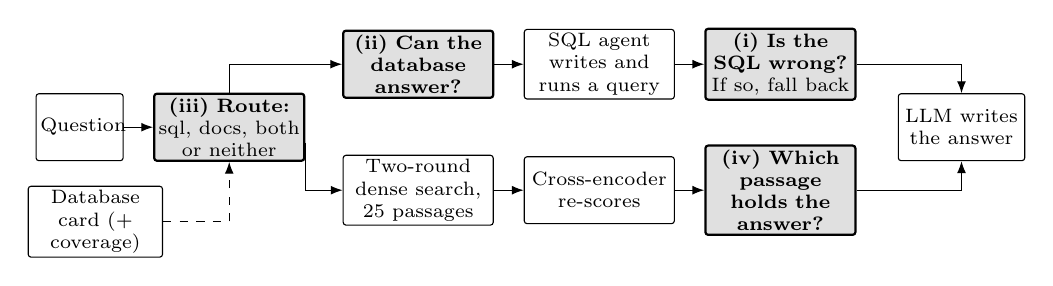
\begin{tikzpicture}[font=\scriptsize, x=1mm, y=1mm,
  box/.style={draw, rounded corners=1pt, align=center, minimum height=8.5mm, inner sep=1.5pt, text width=#1},
  box/.default=18mm,
  dec/.style={box=#1, fill=black!12, thick},
  dec/.default=18mm,
  arr/.style={-{Latex[length=1.5mm]}}]
\node[box=10mm] (q) at (0,0) {Question};
\node[dec=18mm] (route) at (19,0) {\textbf{(iii) Route:} sql, docs, both or neither};
\node[box=16mm] (card) at (2,-12) {Database card (+ coverage)};
\node[dec] (ans) at (43,8) {\textbf{(ii) Can the database answer?}};
\node[box] (sql) at (66,8) {SQL agent writes and runs a query};
\node[dec=18mm] (chk) at (89,8) {\textbf{(i) Is the SQL wrong?} If so, fall back};
\node[box] (dense) at (43,-8) {Two-round dense search, 25 passages};
\node[box] (bge) at (66,-8) {Cross-encoder re-scores};
\node[dec=18mm] (pg) at (89,-8) {\textbf{(iv) Which passage holds the answer?}};
\node[box=15mm] (w) at (112,0) {LLM writes the answer};
\draw[arr] (q) -- (route);
\draw[arr, dashed] (card.east) -| (route.south);
\draw[arr] (route.north) |- (ans.west);
\draw[arr] (route.east) ++(0,-2) |- (dense.west);
\draw[arr] (ans) -- (sql); \draw[arr] (sql) -- (chk);
\draw[arr] (dense) -- (bge); \draw[arr] (bge) -- (pg);
\draw[arr] (chk.east) -| (w.north);
\draw[arr] (pg.east) -| (w.south);
\end{tikzpicture}}
\caption{The assistant under test. Shaded boxes are the four decisions we hand to Jev, each compared with the
component it would replace: (i) an LLM judge or trained verifier (Sect.~\ref{sec:sql}), (ii) word overlap
(Sect.~\ref{sec:answerable}), (iii) an LLM router (Sect.~\ref{sec:routing}), (iv) the cross-encoder's own ranking
(Sect.~\ref{sec:pages}). A two-source question takes both branches.}
\label{fig:pipeline}
\end{figure}

\paragraph{Data.} SQL experiments use the BIRD Mini-Dev questions~\cite{li2023bird} held out from all development
(\N{sN} questions), scored against corrected gold queries~\cite{jin2026annotation}. Routing and page finding use a
database of 23 standard annual figures, taken from SEC XBRL filings, for 31 US companies, together with the 84
filings of FinanceBench's open sample~\cite{islam2023financebench} (44,918 passages). FinanceBench's own questions
served only for development; every result we report as confirmatory comes from questions built after the systems
were frozen.

\paragraph{Jev.} We call \texttt{jev-1.13} through OpenCode Zen at \$0.042 per million input tokens, always
zero-shot, with one fixed question per role. It is never fine-tuned, and its thresholds, where it needs one, are
fitted on separate data.

\paragraph{Use of generative AI.} LLMs wrote the routing and page-finding questions and graded the final answers
(Sects.~\ref{sec:routing}, \ref{sec:pages} and~\ref{sec:e2e}). Generative AI tools also assisted with software
development and with drafting and editing this manuscript. The authors designed the study, checked the results and
take responsibility for the content.

\paragraph{Pre-registration and statistics.} For the answerability, routing, page-finding and end-to-end tests,
hypotheses, measures, tests and thresholds were committed before the data existed, with a change log. The SQL
protocol was committed before its checkers scored the pool but after the companion study scored the first answers;
its hypotheses concern the trained verifier, and every Jev result in it is descriptive. Paired comparisons use the
exact McNemar test (sign-flip permutation for fractional outcomes), one-sided for the SQL hypotheses and two-sided
elsewhere; intervals use 2,000 bootstrap resamples; secondary hypotheses are Holm-corrected. We call two systems \emph{comparable}
only when the 95\% interval of their paired difference lies within $\pm$8 points.

\section{Detecting Wrong SQL and Deciding When to Fall Back}\label{sec:sql}
\paragraph{Setup.} For each question we pooled 21 candidate queries: GPT-5 mini's answer from the pipeline and five
further samples, the same six from gpt-oss-120b, and three samples each from DeepSeek-V4.1-Flash, Qwen3-Coder-30B and
GLM-5.3-Flash. The pipeline's own answer is the \emph{first answer}; it is correct for \N{sFirst} of questions, and
some candidate is correct for \N{sOracle}. Four kinds of checker see the question, the query and a preview of its
result: an LLM judge (Gemini 3.8 Flash, a 0--100 score); ModernBERT-base~\cite{warner2024modernbert} and Laya~\cite{laya2026}, a small
open decision model, each fine-tuned on execution-labelled candidates from other questions; and Jev, zero-shot, asked
``Does this SQL query and its result correctly answer the question?''. Trained checkers are trained, calibrated and
tested on rotating folds stratified by database, so every question is scored by a model that never saw it. The 393
questions, their labels and the first answers are those of the companion study~\cite{companion2026warnings}.



\paragraph{Pre-registered hypotheses.} H1: choosing the candidate with the highest ModernBERT score beats a majority
vote. H2: training on real candidates beats training on rule-based mutants of the reference query. H3: keeping the
first answer unless ModernBERT doubts it, and otherwise choosing from the pool, beats the first answer.



\begin{table}[!htb]
\centering
\caption{Accuracy of answer policies on \N{sN} held-out BIRD questions. Pre-registered comparisons (H1--H3) give wins/losses
and one-sided Holm-adjusted $p$ values; ties among candidates give fractional counts. $\dagger$ = exploratory.}
\label{tab:sql}
\small
\begin{tabular}{@{}l@{\hspace{12pt}}r@{\hspace{12pt}}l@{}}
\toprule
Policy & Acc. & Comparison \\
\midrule
First answer & \N{sFirst} & -- \\
Majority vote (pool) & \N{sVote} & -- \\
ModernBERT-max (H1) & \N{sPfive} & +\N{sH1W}/$-$\N{sH1L}, \N{sH1Pt} \\
ModernBERT-max, mutants (H2) & \N{sPfivem} & \N{sH2Pt} \\
\textbf{ModernBERT cascade (H3)} & \textbf{\N{sPsix}} & +\N{sH3W}/$-$\N{sH3L}, \N{sH3Pt} \\
Jev cascade, $P<0.5^\dagger$ & \N{sJthree} & \N{sJthreeCI} pts \\
Jev-max (pool) & \N{sJevMax} & -- \\
Judge-max (pool) & \N{sJudgeMax} & -- \\
Any candidate right & \N{sOracle} & ceiling \\
\bottomrule
\end{tabular}
\end{table}

\paragraph{Detection.} Zero-shot Jev's AUROC for wrong first answers lies between the LLM judge's and that of
ModernBERT fine-tuned on thousands of labelled candidates (AUROC: LLM judge \N{sAurocJudge}, Jev
\N{sAurocJev}, ModernBERT on real candidates \N{sAurocMB}, Laya fine-tuned \N{sAurocLayaFT}, ModernBERT on mutants
\N{sAurocMBmut}, Laya zero-shot \N{sAurocLayaZS}): the judge's lead is \N{sGapJudgeJev}
(\N{sGapJudgeJevCI}) and Jev's lead over ModernBERT \N{sGapJevMB} (\N{sGapJevMBCI}). Neither difference is
significant, but both intervals are wide: the data do not rule out a judge advantage of about 0.1. Jev's scores are stable: rescoring 200 candidates gave a rank correlation of
\N{sJevRetest}, and scoring all 6,056 distinct candidates cost \N{sJevCost}.

\paragraph{Choosing.} Jev is a much weaker chooser. Taking the candidate it scores highest gives \N{sJevMax} (Table~\ref{tab:sql}), barely
above the first answer and below a plain majority vote (Sect.~\ref{sec:discussion} returns to this).

\paragraph{Falling back.} H3 holds: the ModernBERT-triggered cascade raises accuracy from \N{sFirst} to \N{sPsix}
(gain \N{sPsixCI} points). H1 and H2 point the expected way but are not significant after Holm correction (H2 was significant before it). It falls back on
\N{sPsixFall} of questions (\N{sPsixExtraTok} extra tokens per question, against \N{sCostOtherTok} to build the whole
pool), close to always choosing from the pool (\N{sPfive}). Because Jev doubts well but chooses poorly, we also tried
it as the trigger in front of the best chooser we found (ModernBERT's scores summed within clusters of agreeing
candidates, \N{sPfivev} on every question). With Jev's untuned rule ``fall back when $P(\text{correct})<0.5$'', accuracy reaches \N{sJthree} (gain
\N{sJthreeCI} points) while falling back on only \N{sJthreeFall} of questions (about \N{sJthreeExtraTok} extra tokens
per question); a threshold fitted like H3's gives \N{sJtwo} with \N{sJtwoFall} fallbacks, and Jev as the chooser
gains almost nothing (\N{sJone}). These analyses were decided after the pre-registered ones and are exploratory.

\section{Judging Answerability Against Hard Negatives}\label{sec:answerable}
\paragraph{Setup.} A SQL assistant should decline when its database lacks the data, rather than write a query that
returns something misleading. We took the \N{rthreeN} held-out BIRD questions whose reference query is correct and,
from each query's parse tree, the tables and columns it reads. Each question was paired with three schema cards: its
own database's full schema (answerable), the schema without the tables the query reads, and the schema without the
columns it reads (the hard case: the right tables are still there). Jev was asked ``Does the database described
contain the data needed to answer the question?'', with and without BIRD's hint, which often names columns.

\paragraph{Results.} Jev separates intact schemas from column-removed ones with AUROC \N{rthreeAucCol}
(\N{rthreeAucColCI}) with the hint and \N{rthreeAucColNoHint} (\N{rthreeAucColNoHintCI}) without it, and from
table-removed ones with \N{rthreeAucTab} and \N{rthreeAucTabNoHint}. A deployed gate must, however, almost never
refuse an answerable question. With thresholds fitted on one half of the questions to refuse at most 1\% of
answerable ones and applied to the other half, it refused \N{rthreeFalse} answerable questions while catching
\N{rthreeCatchCol} column-removed and \N{rthreeCatchTab} table-removed ones (with the hint); without the hint, it
caught \N{rthreeCatchColNoHint} and \N{rthreeCatchTabNoHint}. A simple baseline, the share of the
question's words that appear among the card's table and column names (not pre-registered), reaches AUROC
\N{rthreeLexCol} with the hint and \N{rthreeLexColNoHint} without it on the column-removed cards, so Jev's
judgement is far from word matching. Because BIRD repeats some data across tables, a few column-removed cards may
still be answerable and so mislabelled; we did not measure how many.

\section{Routing Between a Database and Documents}\label{sec:routing}
\paragraph{Setup.} We built \N{rtwoN} new questions over the SEC database and the filing library, none from
FinanceBench, with labels fixed by construction: filings only (statements, or figures the database lacks, such as
segment results), either source (a standard annual figure whose filing is in the library), database only in practice
(many companies or years), both, and neither. Five routers, frozen before the set existed, ran once each: an LLM
router (Qwen3.8-27B), a semantic router (majority label of the five most similar earlier questions), Jev asked one
four-way choice under two option wordings written earlier, and Jev asked two yes/no questions (``does answering need
the database?'', ``\ldots the documents?'') with thresholds fitted on an earlier set.

\begin{table}[!htb]
\centering
\caption{Routing on \N{rtwoN} new questions. Per-class columns give correct/total; ``either'' accepts sql or docs.
Latency is the median time to a route.}
\label{tab:routing}
\setlength{\tabcolsep}{3.5pt}
\begin{tabular}{lrrrrrrr}
\toprule
Router & Acc. & Docs & Either & SQL & Hybrid & Neither & Lat. (s) \\
\midrule
LLM router & \N{rtwoLLMAcc} & \N{rtwoLLMDocs} & \N{rtwoLLMEither} & \N{rtwoLLMSql} & \N{rtwoLLMHybrid} & \N{rtwoLLMNeither} & \N{rtwoLLMMs} \\
Semantic (k-NN) & \N{rtwoSemAcc} & \N{rtwoSemDocs} & \N{rtwoSemEither} & \N{rtwoSemSql} & \N{rtwoSemHybrid} & \N{rtwoSemNeither} & -- \\
Jev, choice (wording 1) & \N{rtwoJevOneAcc} & \N{rtwoJevOneDocs} & \N{rtwoJevOneEither} & \N{rtwoJevOneSql} & \N{rtwoJevOneHybrid} & \N{rtwoJevOneNeither} & \N{rtwoJevOneMs} \\
Jev, choice (wording 2) & \N{rtwoJevTwoAcc} & \N{rtwoJevTwoDocs} & \N{rtwoJevTwoEither} & \N{rtwoJevTwoSql} & \N{rtwoJevTwoHybrid} & \N{rtwoJevTwoNeither} & \N{rtwoJevTwoMs} \\
Jev, two yes/no & \N{rtwoJevYNAcc} & \N{rtwoJevYNDocs} & \N{rtwoJevYNEither} & \N{rtwoJevYNSql} & \N{rtwoJevYNHybrid} & \N{rtwoJevYNNeither} & \N{rtwoJevYNMs} \\
\bottomrule
\end{tabular}
\end{table}

\paragraph{Results.} Asked one choice question, Jev routed \N{rtwoJevTwoAcc} of the questions correctly with the
second wording and \N{rtwoJevOneAcc} with the first, against \N{rtwoLLMAcc} for the LLM router
(Table~\ref{tab:routing}); macro-averaged over the five classes the figures are \N{rtwoJevTwoMacro},
\N{rtwoJevOneMacro} and \N{rtwoLLMMacro}. The primary comparison, Jev's second wording against the LLM router, is not significant
(\N{rtwoHoneDiff} points, \N{rtwoHoneCI}, \N{rtwoHoneP}). Its interval reaches past our $\pm$8-point margin, so by
our rule the two are not shown comparable; the data are consistent with Jev being up to about two points worse or
up to ten better. The first
wording is comparable to the LLM router (\N{rtwoHthreeDiff} points, \N{rtwoHthreeCI}). Jev needed no LLM call and
took a median \N{rtwoJevTwoMs}\,s against \N{rtwoLLMMs}\,s.

The routers fail in different places. The LLM router sends most either-source questions to both sources
(\N{rtwoLLMEither} correct), an unneeded search that still reaches the answer; Jev gets those right but sends some
documents-only questions to the database (\N{rtwoJevTwoDocs}), almost all asking for a figure (segment, quarterly or
note) the database does not hold at that detail, and those answers are lost. Counting a route as adequate when it
reaches every source the question needs, the LLM router reaches \N{rtwoLLMCovers} and Jev \N{rtwoJevTwoCovers}.

Posed as two independent yes/no questions, the same model routes \N{rtwoJevYNAcc} correctly, \N{rtwoHtwoDiff} points
below the single choice (\N{rtwoHtwoCI}, \N{rtwoHtwoP}). Its errors go both ways between the two-source class and
the rest: it sends \N{rtwoYNHybToDocs} two-source questions to the documents and \N{rtwoYNHybToSql} to the database,
and \N{rtwoYNEitherToHyb} either-source questions to both. The semantic router, which takes its labels from an earlier set's
examples, reaches only \N{rtwoSemAcc} (\N{rtwoHfourDiff} points against the LLM router, \N{rtwoHfourP}).

One failure is shared by the LLM router and all three Jev routers: each sent the ten questions about companies
that appear in neither source to the database (\N{rtwoLLMNeither} ``neither'' questions right for each, all misses
being these ten); the semantic router declined only \N{rtwoSemNeither}. The router sees the database's columns, not which
companies its rows cover.

\paragraph{Telling the router what the database covers.} We then tested the fix this suggests, pre-registered before its code
existed: a card addition that lists, with no model call, every value of each low-cardinality text column (companies,
tickers, metrics) and each date column's range. On 90 new questions phrased alike in every class (30 about companies
in neither source, 15 about fiscal years 1998--2004, 45 about covered companies and years), coverage raised the share of
uncovered questions that Jev declined from \N{rfourJevOffNeither} to \N{rfourJevOnNeither} (\N{rfourHoneDiff} points,
\N{rfourHoneCI}, \N{rfourHoneP}) and for the LLM router from \N{rfourLLMOffNeither} to \N{rfourLLMOnNeither}
(Holm-adjusted \N{rfourHtwoP}). Unknown companies were almost all caught (\N{rfourJevOnUnknown} and
\N{rfourLLMOnUnknown}); early years mostly were not (\N{rfourJevOnYears} and \N{rfourLLMOnYears}). That subclass is not a clean
test: the card listed a curated table's range (from 2006) beside a raw table's (from 1989).

On covered questions Jev sent all 45 to the database in both arms (acceptable for each, so this check is at its
ceiling); the LLM router improved (\N{rfourHfourDiff} points, \N{rfourHfourCI}, Holm-adjusted \N{rfourHfourP}),
no longer sending most single-figure questions to both sources. Re-run descriptively on the \N{rtwoN} routing
questions, which motivated the change, coverage raised Jev's accuracy from \N{rtwoJevTwoAcc} to
\N{rtwoJevTwoCovAcc} and the LLM router's from \N{rtwoLLMAcc} to \N{rtwoLLMCovAcc}. Each arm was run once.

\section{Finding the Right Page in Long Filings}\label{sec:pages}
\paragraph{Setup.} We sampled pages at random from the 84 filings, at most four per filing, excluding FinanceBench's
evidence pages, a page set used earlier and their neighbours (330 pages from 83 filings, fewer than the 420 planned).
An LLM wrote one specific question per page, and we kept the first \N{roneN} that a second model confirmed the page
answers. For each question the two-round search returned 25 passages twice, once by
dense similarity and once re-scored by the cross-encoder. Four orders were compared: dense similarity (D), the
cross-encoder's scores (B), and Jev's probability that the passage ``contains the information needed to answer the
question'' applied to either list (JD, JB). Only the order differs within a list.

\begin{table}[!htb]
\centering
\caption{Page finding on \N{roneN} new questions: share whose source page is first, in the top 3, and in the top 8
(what the answer writer reads), and share of final answers graded correct when the writer reads those 8
(Sect.~\ref{sec:e2e}).}
\label{tab:pages}
\begin{tabular}{lrrrr}
\toprule
Order & Page@1 & Page@3 & Page@8 & Answer \\
\midrule
Dense similarity (D) & \N{roneDOne} & \N{roneDThree} & \N{roneDEight} & \N{eAD} \\
Cross-encoder, GPU (B) & \N{roneBOne} & \N{roneBThree} & \N{roneBEight} & \N{eAB} \\
Jev over dense (JD) & \N{roneJDOne} & \N{roneJDThree} & \N{roneJDEight} & \N{eAJD} \\
Jev over cross-encoder (JB) & \N{roneJBOne} & \N{roneJBThree} & \N{roneJBEight} & \N{eAJB} \\
\bottomrule
\end{tabular}
\end{table}

\paragraph{Results.} Re-ordering the cross-encoder's 25 passages by Jev put the source page first for \N{roneJBOne} of
questions, against \N{roneBOne} (Table~\ref{tab:pages}; \N{roneHoneDiff} points, \N{roneHoneCI}, \N{roneHoneP}), and
raised the top-three share (\N{roneHfourDiff} points, \N{roneHfourP}). Over the dense list alone, without a GPU, Jev
reached \N{roneJDOne}: \N{roneHthreeDiff} points above dense similarity (\N{roneHthreeP}) and \N{roneHtwoDiff} above
the cross-encoder, just short of significance (\N{roneHtwoCI}, \N{roneHtwoP}). The gain is at the top: the share with
the source page among the eight passages the writer reads rises only from \N{roneBEight} to \N{roneJBEight}, and no
order can exceed \N{roneBInList}. Resampling the \N{roneFilings} filings instead of questions leaves the main interval
almost unchanged (\N{roneHoneCIFiling}; post hoc).


Scoring one question's 25 passages took Jev a median \N{roneJevMs}\,ms (eight requests at a time) and cost
\N{roneCost}; the search took \N{roneDenseMs}\,ms without re-ranking and \N{roneBgeMs}\,ms with the cross-encoder, on
a GPU shared with other jobs.

\section{From Decisions to Final Answers}\label{sec:e2e}
\paragraph{Setup.} Two pre-registered tests ask whether these gains reach the final answer. First, the pipeline's answer writer (gpt-oss-120b) answered each of the \N{eAN} page questions four
times, reading the first eight passages of each order in Table~\ref{tab:pages}. Second, the \N{eBN} routing
questions were asked through the assistant's API with Jev on (Jev routes and re-ranks) and off (the LLM router
routes; passages keep the search order). An LLM grader (Gemini 3.8 Flash, one fixed prompt, blind to the arm)
compared each answer with a reference: the page or documents answer, the reference query's result (for two-source
questions, the database figure only), or a refusal where neither source can answer. No answer was graded by hand.


\paragraph{Page order.} The page-finding gains over the cross-encoder do not reach the answer when the writer reads
eight passages. Re-ordering the cross-encoder's list with Jev left answer accuracy unchanged (\N{eAJB} against
\N{eAB}; \N{eAoneDiff} points, \N{eAoneCI}, \N{eAoneP}). Over the dense list, by contrast, Jev raised accuracy from
\N{eAD} to \N{eAJD} (\N{eAtwoDiff} points, \N{eAtwoCI}, Holm-adjusted \N{eAtwoP}), level with the GPU cross-encoder
(\N{eAthreeDiff} points, \N{eAthreeCI}; Table~\ref{tab:pages}, last column). What decides the answer is whether the source page is among the eight passages
at all (with the cross-encoder's order, \N{eABIn} of answers were correct when it was and \N{eABOut} when not). At the
answer level, Jev's value is replacing the GPU re-ranker at no loss, not improving on it.


\paragraph{The whole assistant.} With Jev on, the assistant answered \N{eBOn} of the routing questions correctly,
against \N{eBOff} with it off (\N{eBoneDiff} points, \N{eBoneCI}, \N{eBoneP}; +\N{eBoneW}/$-$\N{eBoneL}). Both declined
all questions neither source can answer (\N{eBOnNeither} and \N{eBOffNeither}). (\N{eBFallback} Jev-arm questions fell back to the LLM router when the Jev
call failed and stay in, as registered.) The difference is concentrated in two-source questions (\N{eBOnHybrid} against
\N{eBOffHybrid}), although both arms chose the same route for all of them. The LLM router also
writes the database part of a two-source question as its own question (\N{eBSplitLLM} in the routing test); Jev only
chooses (\N{eBSplitJev}), so the SQL agent receives the whole compound question and, in the answers we read,
reported the figure as unavailable. Documents-only questions went the
other way (\N{eBOnDocs} against \N{eBOffDocs}). A Jev router therefore needs its own split of
two-source questions; until it has one, its speed costs accuracy on them.

\section{Discussion}\label{sec:discussion}
\paragraph{Reading off versus working out.} Li et al.\ found that Jev judges as well as a frontier model when a
verdict can be read off the text and falls behind when it must be derived~\cite{li2026jevjudge}. Our results fit
that pattern: Jev did best where the answer is visible in the input (whether a passage states a figure, whether a
schema has the needed columns, whether a result looks plausible) and worst where it must be worked out (which of two
plausible queries is right). This is an interpretation we did not
isolate (the tasks also differ in format and wording); if it holds, a decision model is better used to
\emph{trigger} work (fall back, re-rank, decline) than to \emph{choose} among generated answers.

\paragraph{Ask one question, not two.} Routing is one decision with four outcomes; split into
``needs the database?'' and ``needs the documents?'', each probability is reasonable alone, but the pair does not
separate questions that need both sources from those either can answer. This fits the over-endorsement of single statements reported for
Jev~\cite{axioms2026}, though our wording may also contribute: when either source suffices, neither is strictly
``needed''. Posed as two questions, the decision cost \N{rtwoHtwoDiff} points; one choice removed it.


\paragraph{Calibration and cost.} Post hoc, Jev's probability for its chosen route averaged \N{calRouteMeanP} against an accuracy of \N{calRouteObs} (expected calibration error
\N{calRouteEce}; routes given at least 0.9 were right \N{calRouteTopObs} of the time), so it could serve directly as a
threshold for escalating to an LLM (untested). Passage scores rank well (AUROC \N{calPageAuroc}) but are poor absolute
probabilities: passages scored at least 0.9 lay on the source page only \N{calPageTopObs} of the time (an
underestimate, as other pages may also answer), so they should only order passages.
A Jev routing call used \N{costJevIn} input tokens and took \N{costJevMs}\,s, against \N{costLLMIn} input and
\N{costLLMOut} output tokens and \N{costLLMMs}\,s for the LLM router; re-ranking costs are in Sect.~\ref{sec:pages}.
We did not measure the cost of hosting the LLM router or the cross-encoder's GPU.



\section{Threats to Validity}\label{sec:threats}
\paragraph{Questions and labels.} The routing and page questions were generated, from templates and by an LLM,
and may be cleaner than real users' questions, which we have not tested. A page other than the source page may also
answer a question, which lowers every order's page accuracy alike. Both Jev routing wordings
were frozen before the new set existed, though the second followed an earlier test of the first. Routing labels are fixed by construction,
and a page question was kept only when a second model confirmed its page answers it. A model not otherwise used here
(GPT-6.1 Sol) agreed with 37 of 40 sampled routing labels ($\kappa=0.90$) and accepted all 30 sampled page questions;
no sample was labelled by hand.
\paragraph{Wording and grading.} Each Jev role used one fixed wording (two for routing); accuracy of typed decision
models moves by about five points with wording~\cite{fastslow2026}, our two routing wordings differed by
\N{rtwoJevTwoAcc} against \N{rtwoJevOneAcc}, and we did not test paraphrased questions. The end-to-end tests were
graded by an LLM with no human check, asked each question once per arm, and graded two-source answers on their
database figure only.
\paragraph{Scope.} BIRD for SQL, one financial database and one filing library for the rest, English only; other
domains, document types and languages are untested. Jev is a commercial model whose training data we do not know, and
the models may have seen BIRD. Earlier, weaker versions of the
page-finding and routing tests were replaced by the pre-registered ones reported here.

\section{Conclusion}
Zero-shot on held-out data, a typed decision model detected wrong SQL answers with an AUROC not significantly different from an LLM judge's,
ranked schemas by answerability (AUROC \N{rthreeAucCol}), routed \N{rtwoJevTwoAcc} of new questions right without an
LLM call, and put the right page first more often than a cross-encoder (\N{roneJBOne} against \N{roneBOne}); it
chose poorly among SQL candidates and failed when one routing decision was split in two. End to end, Jev's
page order matched a GPU cross-encoder's answer accuracy without a GPU but did not improve on it, and an assistant
using Jev was not significantly less accurate than one routed by an LLM, losing most on two-source questions, which
need the split of the question that the LLM router provides. The next steps are human grading of final answers, tests on
real users' questions and on other domains and languages, and checks of robustness to rewording. Code, prompts,
pre-registrations, question sets and result files are available from the authors on request.

\begin{credits}
\subsubsection{\discintname}
The authors have no competing interests to declare that are relevant to the content of this article.
\end{credits}

\bibliographystyle{splncs04}
\bibliography{refs}
\end{document}
